\documentclass[tikz,border=10pt]{standalone}
\usepackage{ctex} % 如需中文支持
\usetikzlibrary{intersections, calc}

\begin{document}

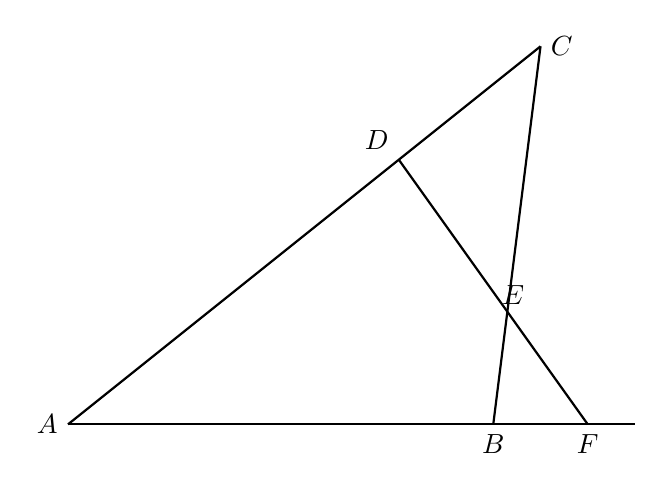
\begin{tikzpicture}[>=stealth, thick, scale=1.2]
    % 1. 定义核心顶点坐标 (根据原图视觉比例设定)
    \coordinate (A) at (0,0);
    \coordinate (C) at (5,4);
    \coordinate (B) at (4.5,0);
    
    % 2. 定义辅助路径用于求交点
    % 线段 AC
    \path[name path=AC] (A) -- (C);
    % 延长线 AB 所在的直线
    \path[name path=lineAB] (A) -- (6,0);
    
    % 3. 设定点 D 在 AC 上，点 F 在 AB 延长线上
    \coordinate (D) at ($(A)!0.7!(C)$); % D点位于AC上约70%处
    \coordinate (F) at (5.5,0);          % F点在AB右侧的延长线上
    
    % 4. 连结 DF 并定义为路径，用于计算与 BC 的交点 E
    \path[name path=DF] (D) -- (F);
    \path[name path=BC] (B) -- (C);
    
    % 使用 intersections 库自动计算交点 E
    \fill [name intersections={of=DF and BC, by=E}];

    % 5. 绘制所有实线段
    \draw (A) -- (C);          % 边 AC
    \draw (A) -- (6,0);        % 射线 AB 及其延长向右
    \draw (B) -- (C);          % 线段 BC
    \draw (D) -- (F);          % 线段 DF

    % 6. 标注文本标签
    % 调整锚点(anchor)确保标注不遮挡线条
    \node[left] at (A) {$A$};
    \node[right] at (C) {$C$};
    \node[below] at (B) {$B$};
    \node[above left] at (D) {$D$};
    \node[right=2pt, above=-1pt] at (E) {$E$};
    \node[below] at (F) {$F$};

    % 7. 可选：标记已知点 (小圆点)
    %\foreach \p in {A,B,C,D,E,F} \fill (\p) circle (1pt);

\end{tikzpicture}

\end{document}